% Options for packages loaded elsewhere
\PassOptionsToPackage{unicode}{hyperref}
\PassOptionsToPackage{hyphens}{url}
%
\documentclass[
  12pt,
]{article}
\usepackage{amsmath,amssymb}
\usepackage{iftex}
\ifPDFTeX
  \usepackage[T1]{fontenc}
  \usepackage[utf8]{inputenc}
  \usepackage{textcomp} % provide euro and other symbols
\else % if luatex or xetex
  \usepackage{unicode-math} % this also loads fontspec
  \defaultfontfeatures{Scale=MatchLowercase}
  \defaultfontfeatures[\rmfamily]{Ligatures=TeX,Scale=1}
\fi
\usepackage{lmodern}
\ifPDFTeX\else
  % xetex/luatex font selection
\fi
% Use upquote if available, for straight quotes in verbatim environments
\IfFileExists{upquote.sty}{\usepackage{upquote}}{}
\IfFileExists{microtype.sty}{% use microtype if available
  \usepackage[]{microtype}
  \UseMicrotypeSet[protrusion]{basicmath} % disable protrusion for tt fonts
}{}
\makeatletter
\@ifundefined{KOMAClassName}{% if non-KOMA class
  \IfFileExists{parskip.sty}{%
    \usepackage{parskip}
  }{% else
    \setlength{\parindent}{0pt}
    \setlength{\parskip}{6pt plus 2pt minus 1pt}}
}{% if KOMA class
  \KOMAoptions{parskip=half}}
\makeatother
\usepackage{xcolor}
\usepackage[margin=1in]{geometry}
\usepackage{longtable,booktabs,array}
\usepackage{calc} % for calculating minipage widths
% Correct order of tables after \paragraph or \subparagraph
\usepackage{etoolbox}
\makeatletter
\patchcmd\longtable{\par}{\if@noskipsec\mbox{}\fi\par}{}{}
\makeatother
% Allow footnotes in longtable head/foot
\IfFileExists{footnotehyper.sty}{\usepackage{footnotehyper}}{\usepackage{footnote}}
\makesavenoteenv{longtable}
\usepackage{graphicx}
\makeatletter
\def\maxwidth{\ifdim\Gin@nat@width>\linewidth\linewidth\else\Gin@nat@width\fi}
\def\maxheight{\ifdim\Gin@nat@height>\textheight\textheight\else\Gin@nat@height\fi}
\makeatother
% Scale images if necessary, so that they will not overflow the page
% margins by default, and it is still possible to overwrite the defaults
% using explicit options in \includegraphics[width, height, ...]{}
\setkeys{Gin}{width=\maxwidth,height=\maxheight,keepaspectratio}
% Set default figure placement to htbp
\makeatletter
\def\fps@figure{htbp}
\makeatother
\setlength{\emergencystretch}{3em} % prevent overfull lines
\providecommand{\tightlist}{%
  \setlength{\itemsep}{0pt}\setlength{\parskip}{0pt}}
\setcounter{secnumdepth}{5}
\usepackage[OT4]{polski}
\usepackage[utf8]{inputenc}
\usepackage{graphicx}
\usepackage{float}
\usepackage{xcolor}
\usepackage{booktabs}
\usepackage{longtable}
\usepackage{array}
\usepackage{multirow}
\usepackage{wrapfig}
\usepackage{float}
\usepackage{colortbl}
\usepackage{pdflscape}
\usepackage{tabu}
\usepackage{threeparttable}
\usepackage{threeparttablex}
\usepackage[normalem]{ulem}
\usepackage{makecell}
\usepackage{xcolor}
\ifLuaTeX
  \usepackage{selnolig}  % disable illegal ligatures
\fi
\usepackage{bookmark}
\IfFileExists{xurl.sty}{\usepackage{xurl}}{} % add URL line breaks if available
\urlstyle{same}
\hypersetup{
  pdftitle={Sprawozdanie 2},
  pdfauthor={Kacper Szmigielski, 282255 i Mateusz Wizner},
  hidelinks,
  pdfcreator={LaTeX via pandoc}}

\title{Sprawozdanie 2}
\usepackage{etoolbox}
\makeatletter
\providecommand{\subtitle}[1]{% add subtitle to \maketitle
  \apptocmd{\@title}{\par {\large #1 \par}}{}{}
}
\makeatother
\subtitle{Eksploracja danych}
\author{Kacper Szmigielski, 282255 i Mateusz Wizner}
\date{2025-04-26}

\begin{document}
\maketitle

{
\setcounter{tocdepth}{3}
\tableofcontents
}
\begin{verbatim}
##   X     UA_Name   UA_Country  UA_Continent Housing Cost.of.Living Startups
## 1 0      Aarhus      Denmark        Europe  6.1315          4.015   2.8270
## 2 1    Adelaide    Australia       Oceania  6.3095          4.692   3.1365
## 3 2 Albuquerque   New Mexico North America  7.2620          6.059   3.7720
## 4 3      Almaty   Kazakhstan          Asia  9.2820          9.333   2.4585
## 5 4   Amsterdam  Netherlands        Europe  3.0530          3.824   7.9715
## 6 5   Anchorage       Alaska North America  5.4335          3.141   2.7945
##   Venture.Capital Travel.Connectivity Commute Business.Freedom Safety
## 1           2.512              3.5360 6.31175         9.940000 9.6165
## 2           2.640              1.7765 5.33625         9.399667 7.9260
## 3           1.493              1.4555 5.05575         8.671000 1.3435
## 4           0.000              4.5920 5.87125         5.568000 7.3090
## 5           6.107              8.3245 6.11850         8.836667 8.5035
## 6           0.000              1.7380 4.71525         8.671000 3.4705
##   Healthcare Education Environmental.Quality Economy Taxation Internet.Access
## 1   8.704333    5.3665               7.63300  4.8865   5.0680          8.3730
## 2   7.936667    5.1420               8.33075  6.0695   4.5885          4.3410
## 3   6.430000    4.1520               7.31950  6.5145   4.3460          5.3960
## 4   4.545667    2.2830               3.85675  5.2690   8.5220          2.8860
## 5   7.907333    6.1800               7.59725  5.0530   4.9550          4.5230
## 6   6.060333    3.6245               9.27200  6.5145   4.7720          4.9645
##   Leisure...Culture Tolerance Outdoors
## 1            3.1870    9.7385   4.1300
## 2            4.3285    7.8220   5.5310
## 3            4.8900    7.0285   3.5155
## 4            2.9370    6.5395   5.5000
## 5            8.8740    8.3680   5.3070
## 6            3.2660    7.0930   5.3580
\end{verbatim}

\begin{verbatim}
## Warning: pakiet 'dplyr' został zbudowany w wersji R 4.4.2
\end{verbatim}

\begin{verbatim}
## Warning: pakiet 'kableExtra' został zbudowany w wersji R 4.4.3
\end{verbatim}

\begin{verbatim}
## Warning: pakiet 'patchwork' został zbudowany w wersji R 4.4.2
\end{verbatim}

\begin{verbatim}
## Warning: pakiet 'arules' został zbudowany w wersji R 4.4.3
\end{verbatim}

\begin{verbatim}
## Warning: pakiet 'e1071' został zbudowany w wersji R 4.4.3
\end{verbatim}

\section{ZADANIE 1 (Dyskretyzacja(przedziałowanie) cech
ciągłych)}\label{zadanie-1-dyskretyzacjaprzedziaux142owanie-cech-ciux105gux142ych}

\subsection{a) Dane: iris (R-pakiet
datasets).}\label{a-dane-iris-r-pakiet-datasets.}

\textbf{3} Pierwsze wiersze z pakietu iris

\begin{longtable}[]{@{}rrrrl@{}}
\toprule\noalign{}
Sepal.Length & Sepal.Width & Petal.Length & Petal.Width & Species \\
\midrule\noalign{}
\endhead
\bottomrule\noalign{}
\endlastfoot
5.1 & 3.5 & 1.4 & 0.2 & setosa \\
4.9 & 3.0 & 1.4 & 0.2 & setosa \\
4.7 & 3.2 & 1.3 & 0.2 & setosa \\
\end{longtable}

Zbiór danych zawiera wyniki pomiarów uzyskanych dla \textbf{trzech
gatunków irysów} (tj. setosa, versicolor i virginica) i został
\textbf{udostępniony przez Ronalda Fishera w roku 1936.}

-- \textbf{Pomiary} dotyczą \textbf{długości oraz szerokości} dwóch
różnych części kwiatu-- działki \textbf{kielicha (ang. sepal) oraz
płatka (ang. petal).}

\subsection{b) Wybór cech}\label{b-wybuxf3r-cech}

Cechy, inaczej właściwie możemy to rozstrzygać jako kolumny, które
charakteryzują się \textbf{największym zróżnicowaniem} w stosunku do
rodzaju gatunku

\begin{center}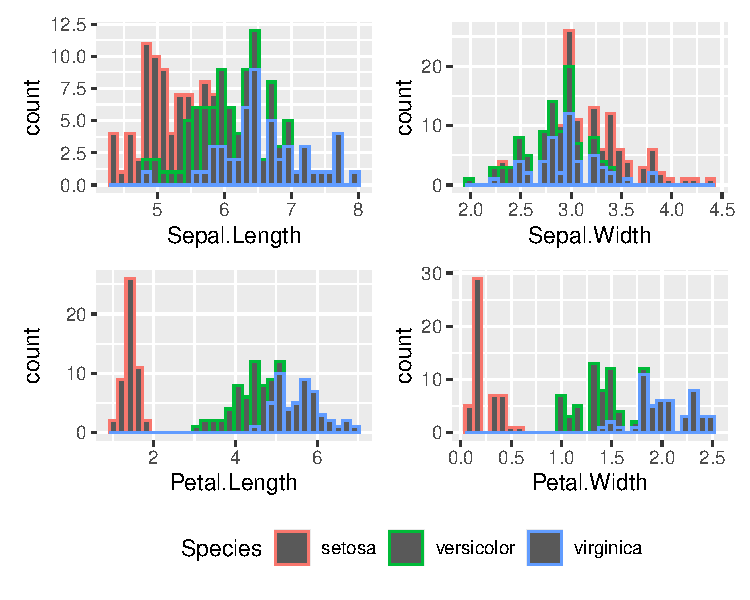
\includegraphics{Sprawozdanie2_files/figure-latex/zad1b-1} \end{center}

Po przeanalizowaniu histogramów, widać ,że warto zwrócić uwagę na takie
cechy jak \textbf{Petal.Length i Petal.Width}, ponieważ

widać dobrze zaznaczone przedziały w których występuje większość
kwiatków danego gatunku.

Dalej warto jest też spojrzeć na to jak nasze \emph{obserwawcje}
teoretycznie rozkładają się w przestrzeni 2D, aby to zrobić dodajemy
jedną dodatkową kolumnę y, wypełnioną losowymi liczbami od 0 do 1
(rozkłąd jednostajny)

\begin{center}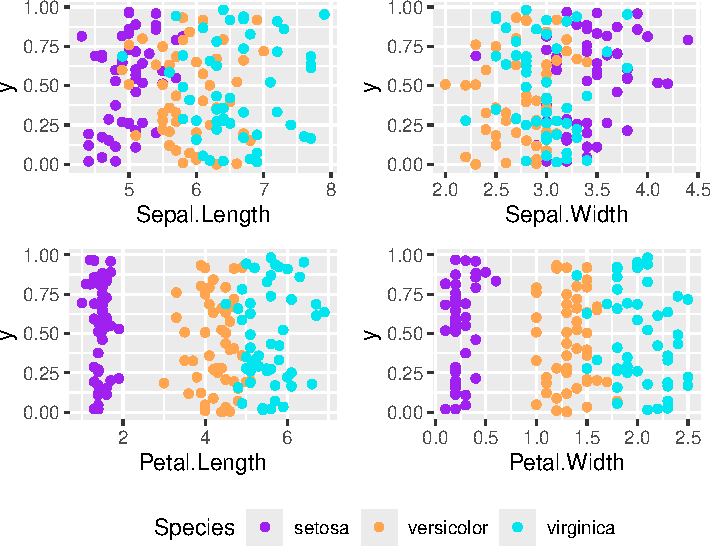
\includegraphics{Sprawozdanie2_files/figure-latex/zad1b1-1} \end{center}

Wykresy typu scatter-plot potwierdzają ,że \textbf{Petal.Length i
Petal.Width} są bardzo dobry wyborem cech, które mogłyby być
wyznacznikami gatunków roślin.

Musimy jednak wybrać wartości najlepsze i najgorsze, aby to zrobić
przeanalizujemy jeszcze boxploty.

\begin{center}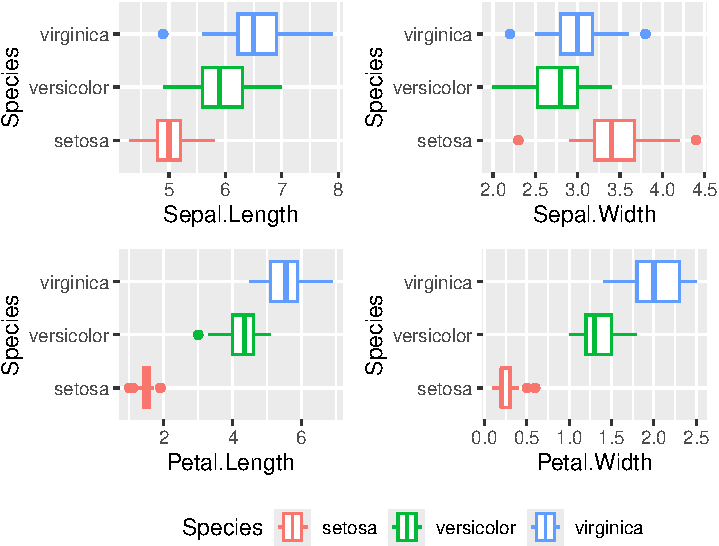
\includegraphics{Sprawozdanie2_files/figure-latex/zad1b2-1} \end{center}

Na ich podstawaie możemy uznać, że Petal.Width może stanowić najlepszy
wyznacznik gatunku roślin Najgorszym natomiast jest Sepal.Width, tutaj
duża część gatunków dzieli te same wartości tej cechy.

\subsection{c) Porównanie nienadzorowanych metod
dyskretyzacji}\label{c-poruxf3wnanie-nienadzorowanych-metod-dyskretyzacji}

\subsubsection{Równe częstości}\label{ruxf3wne-czux119stoux15bci}

\paragraph{Dla najlepszej}\label{dla-najlepszej}

\begin{center}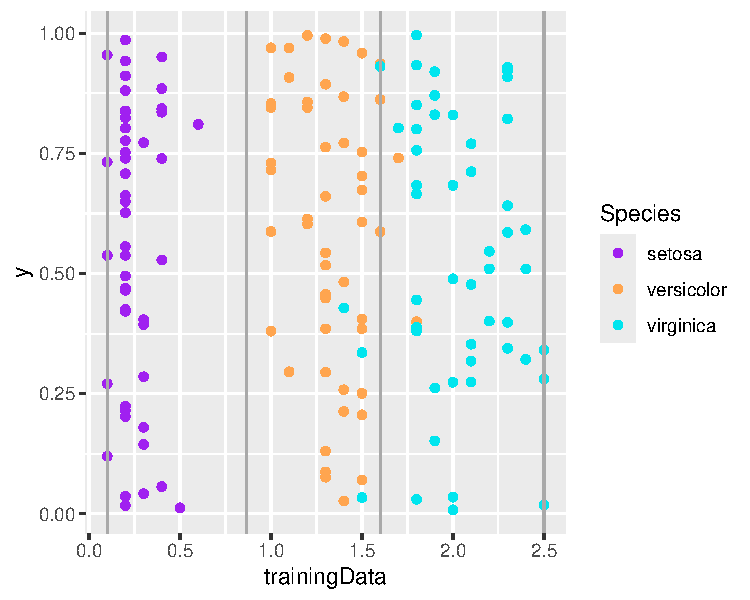
\includegraphics{Sprawozdanie2_files/figure-latex/frequences_najl-1} \end{center}

\begin{center}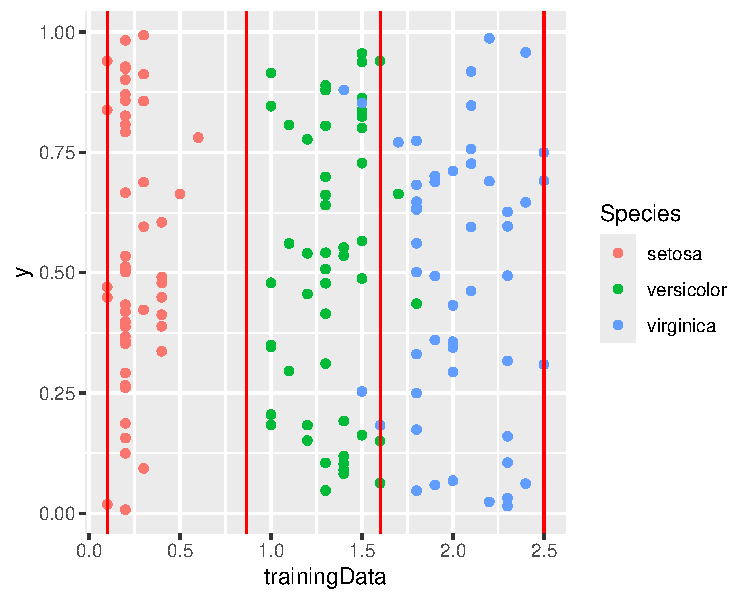
\includegraphics{Sprawozdanie2_files/figure-latex/frequences_najl-2} \end{center}

\begin{center}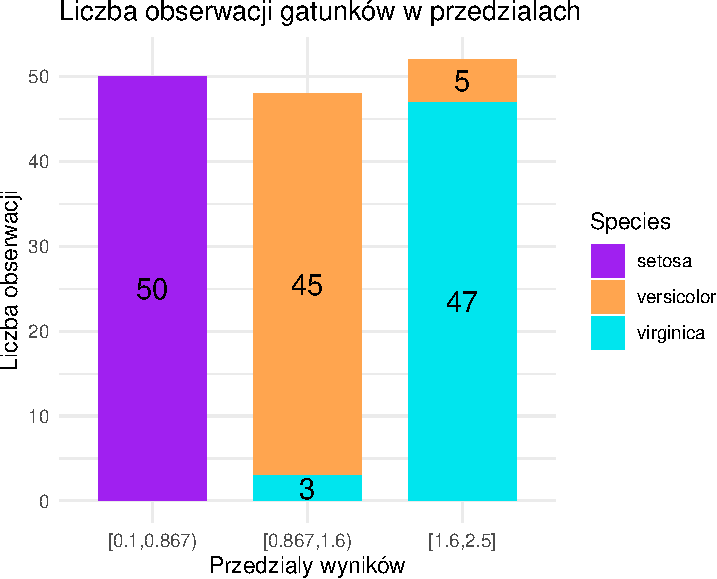
\includegraphics{Sprawozdanie2_files/figure-latex/tabela_kondygnacji_1_najl-1} \end{center}

\begin{verbatim}
##           [,1]
## [1,] 0.9466667
\end{verbatim}

\paragraph{Dla najgorszej}\label{dla-najgorszej}

\begin{center}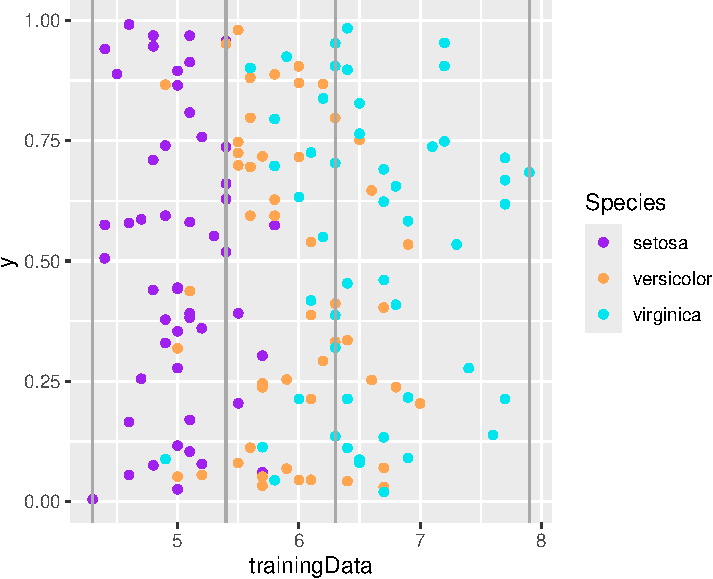
\includegraphics{Sprawozdanie2_files/figure-latex/frequences_najg-1} \end{center}

\begin{center}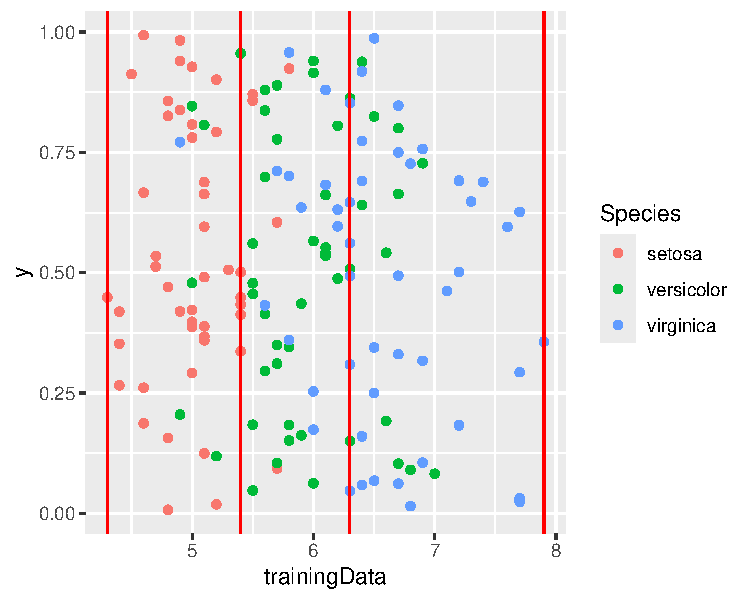
\includegraphics{Sprawozdanie2_files/figure-latex/frequences_najg-2} \end{center}

\begin{center}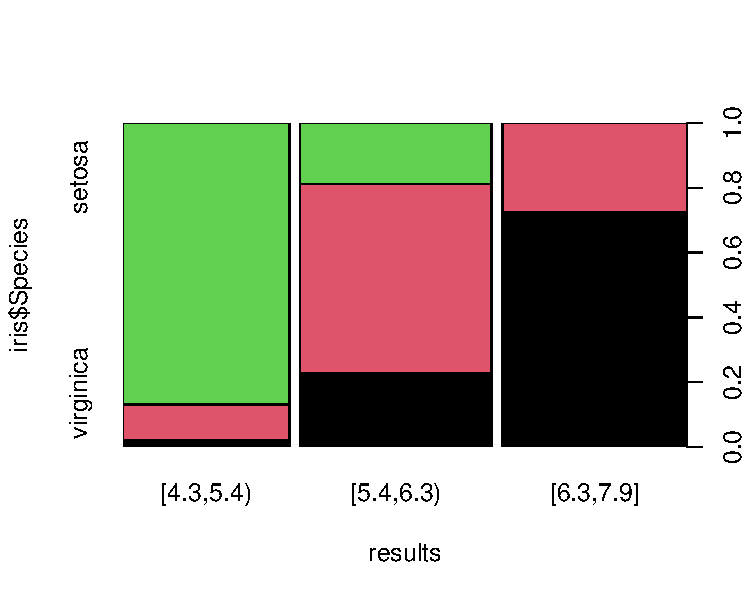
\includegraphics{Sprawozdanie2_files/figure-latex/tabela_kondygnacji_1_najg-1} \end{center}

\begin{verbatim}
##      [,1]
## [1,] 0.72
\end{verbatim}

\subsubsection{Równe szerokości}\label{ruxf3wne-szerokoux15bci}

\paragraph{Dla najlepszej}\label{dla-najlepszej-1}

\begin{center}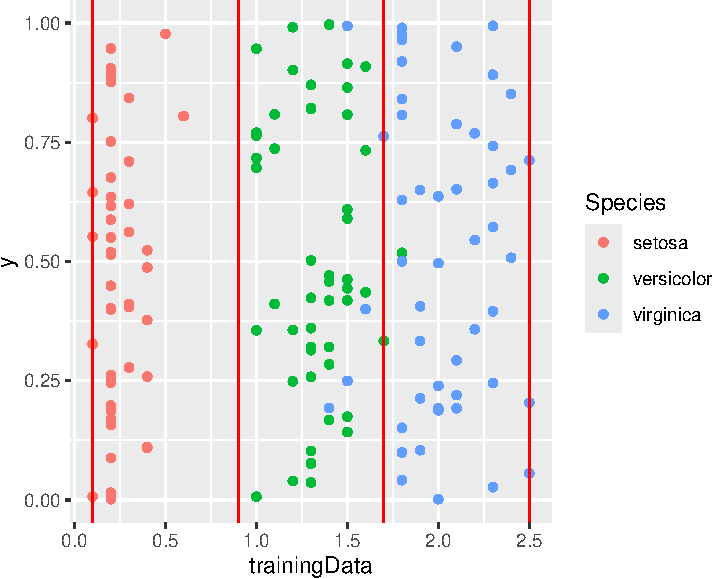
\includegraphics{Sprawozdanie2_files/figure-latex/width_najl-1} \end{center}

\begin{center}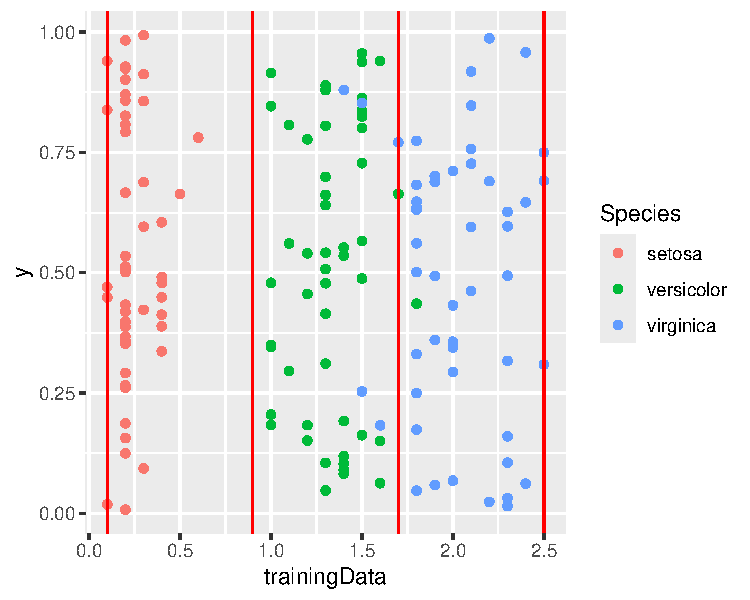
\includegraphics{Sprawozdanie2_files/figure-latex/width_najl-2} \end{center}

\begin{center}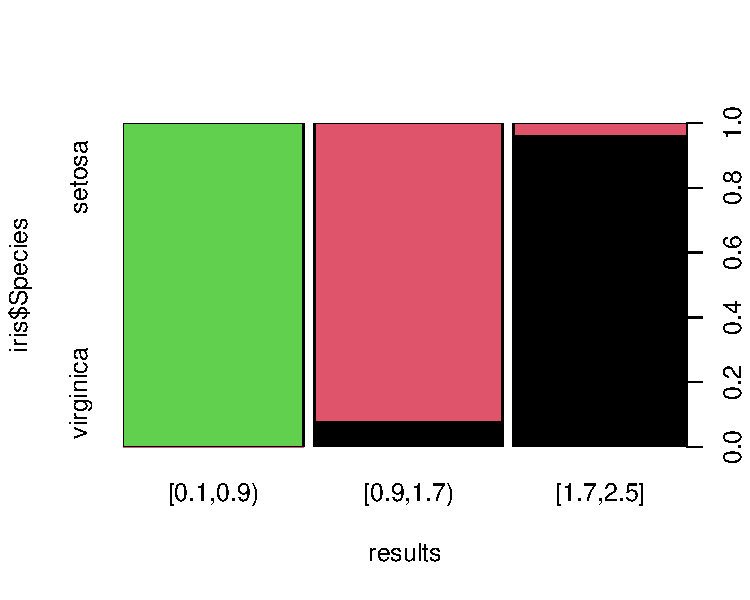
\includegraphics{Sprawozdanie2_files/figure-latex/tabela_kondygnacji_2_najl-1} \end{center}

\begin{verbatim}
##      [,1]
## [1,] 0.96
\end{verbatim}

\paragraph{Dla najgorszej}\label{dla-najgorszej-1}

\begin{center}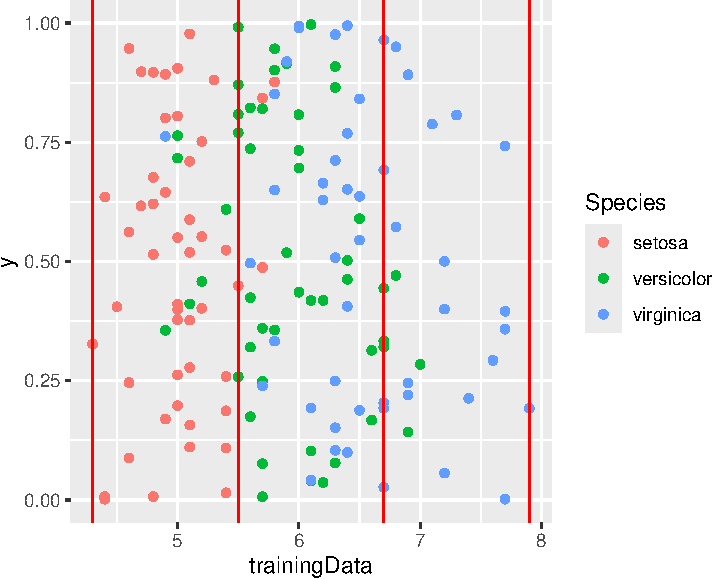
\includegraphics{Sprawozdanie2_files/figure-latex/width_najg-1} \end{center}

\begin{center}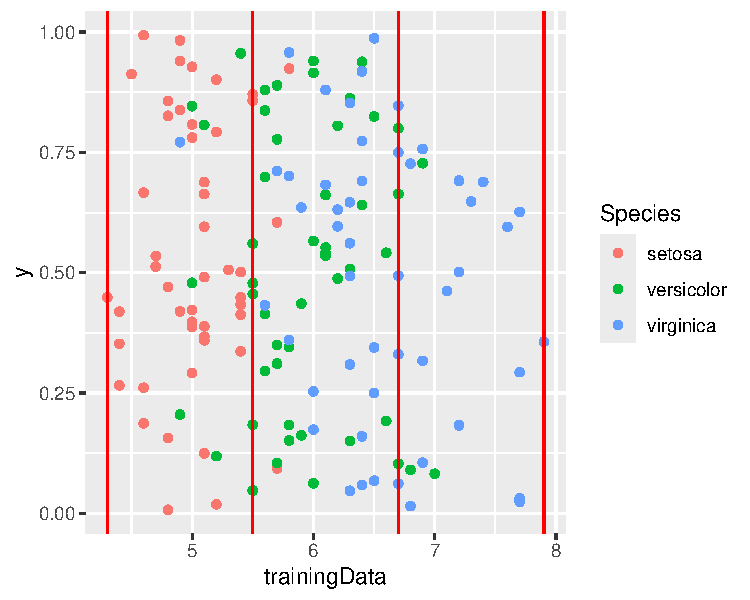
\includegraphics{Sprawozdanie2_files/figure-latex/width_najg-2} \end{center}

\begin{center}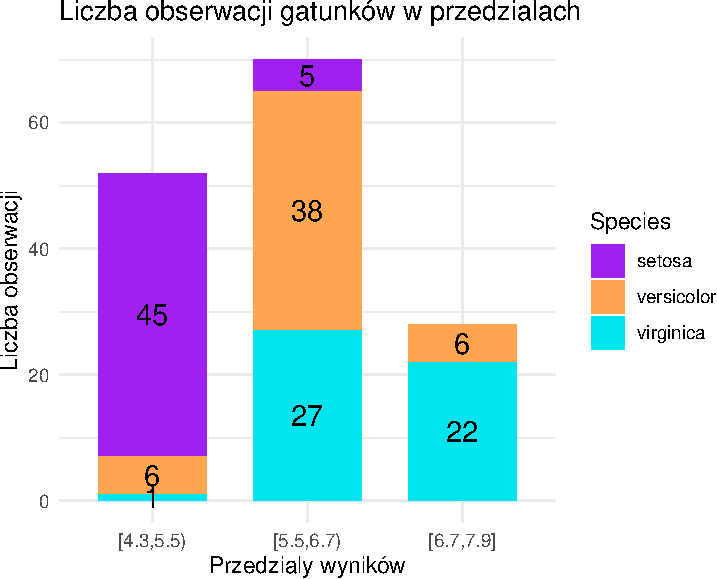
\includegraphics{Sprawozdanie2_files/figure-latex/tabela_kondygnacji_2_najg-1} \end{center}

\begin{verbatim}
##           [,1]
## [1,] 0.5729167
\end{verbatim}

\subsubsection{K-means}\label{k-means}

\paragraph{Dla najlepszej}\label{dla-najlepszej-2}

\begin{center}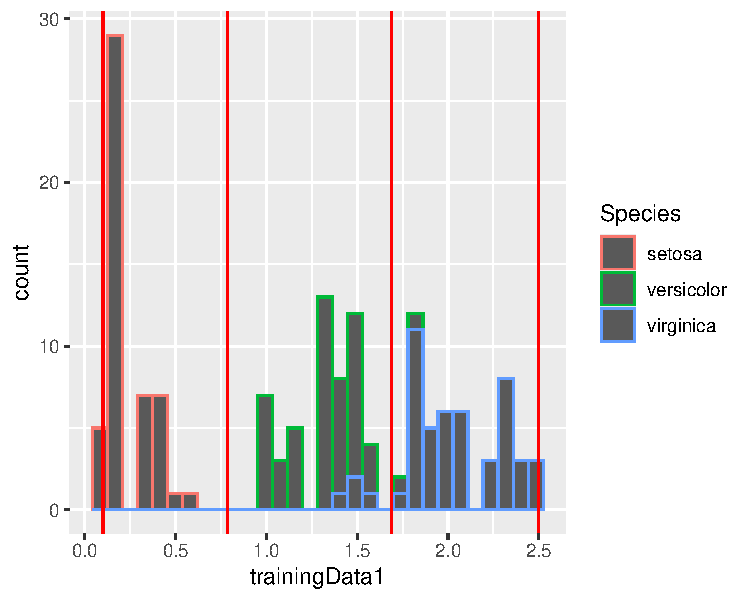
\includegraphics{Sprawozdanie2_files/figure-latex/kMeans_najl-1} \end{center}

\begin{center}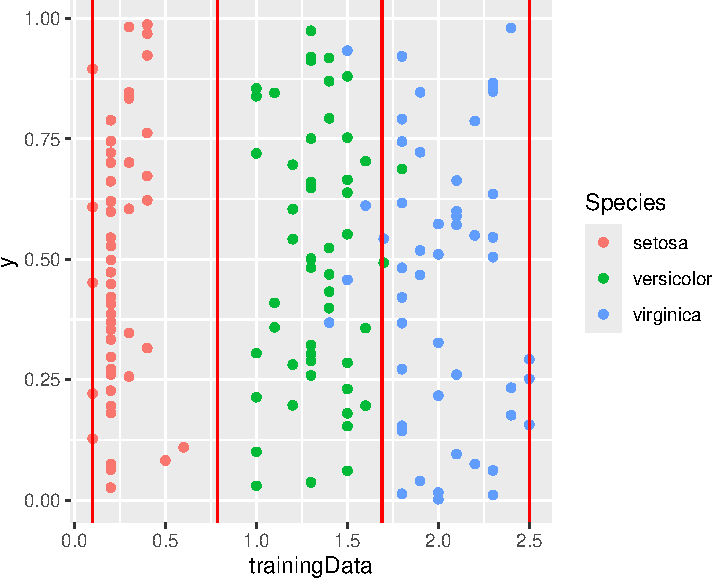
\includegraphics{Sprawozdanie2_files/figure-latex/kMeans_najl-2} \end{center}

\begin{center}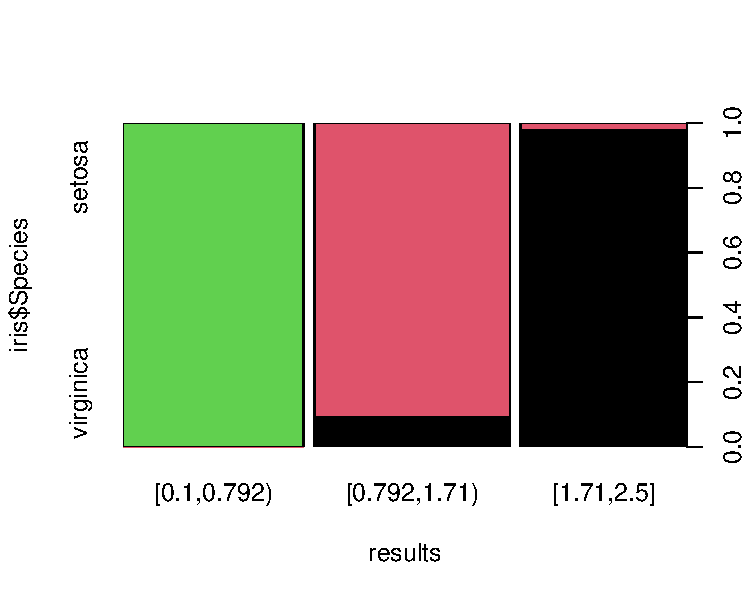
\includegraphics{Sprawozdanie2_files/figure-latex/tabela_kondygnacji_3_najl-1} \end{center}

\begin{verbatim}
##      [,1]
## [1,] 0.96
\end{verbatim}

\paragraph{Dla najgorszej}\label{dla-najgorszej-2}

\begin{center}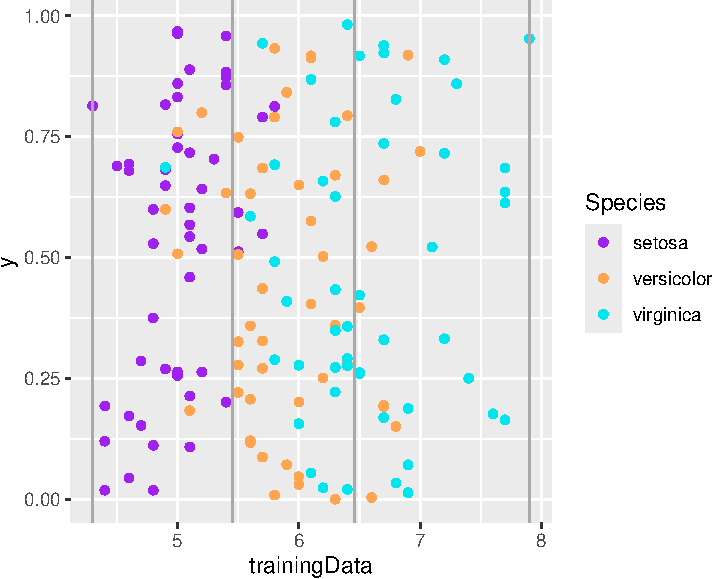
\includegraphics{Sprawozdanie2_files/figure-latex/kMeans_najg-1} \end{center}

\begin{center}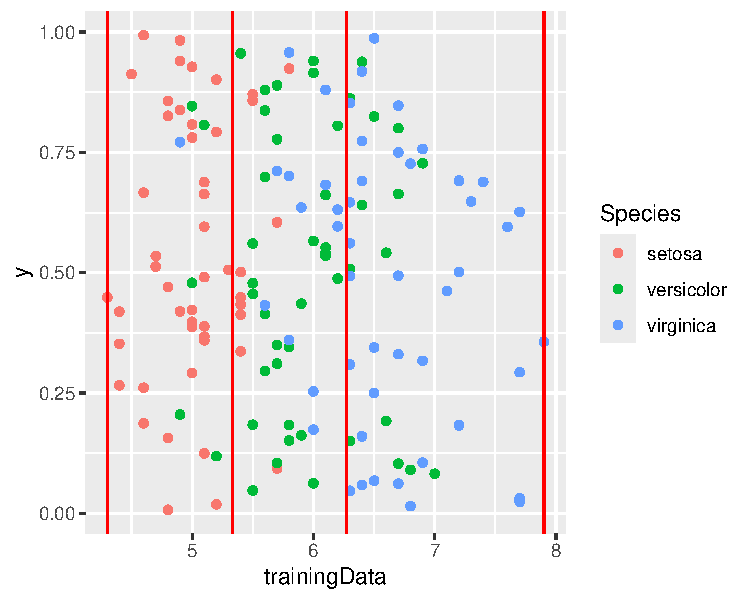
\includegraphics{Sprawozdanie2_files/figure-latex/kMeans_najg-2} \end{center}

\begin{center}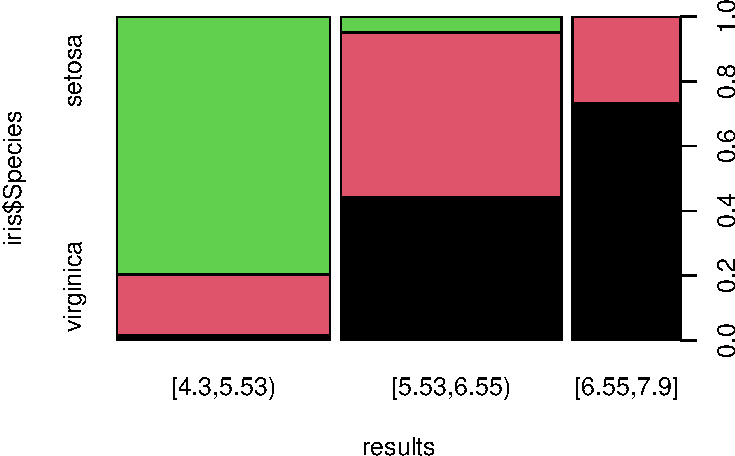
\includegraphics{Sprawozdanie2_files/figure-latex/tabela_kondygnacji_3_najg-1} \end{center}

\begin{verbatim}
## [1] 0.72
\end{verbatim}

\subsubsection{Dyskretyzacja z przedziałami zadanymi przez
urzytkownika}\label{dyskretyzacja-z-przedziaux142ami-zadanymi-przez-urzytkownika}

\paragraph{Dla najlepszej}\label{dla-najlepszej-3}

\begin{center}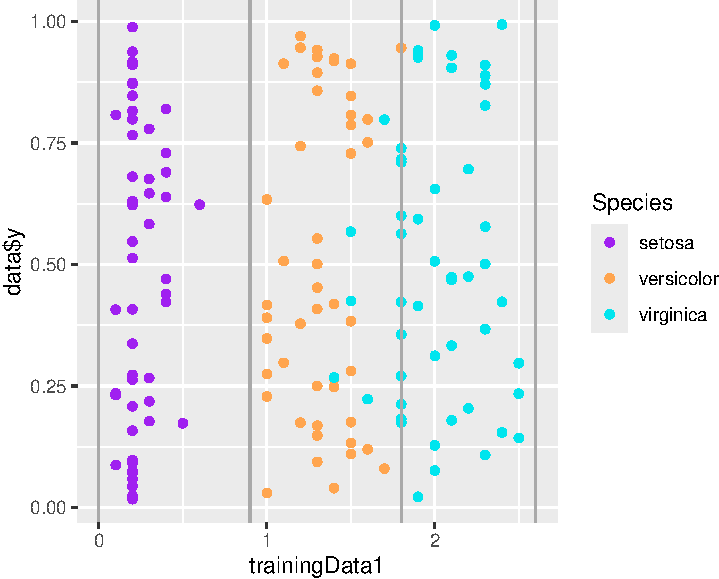
\includegraphics{Sprawozdanie2_files/figure-latex/givenRanges_najl-1} \end{center}

\begin{center}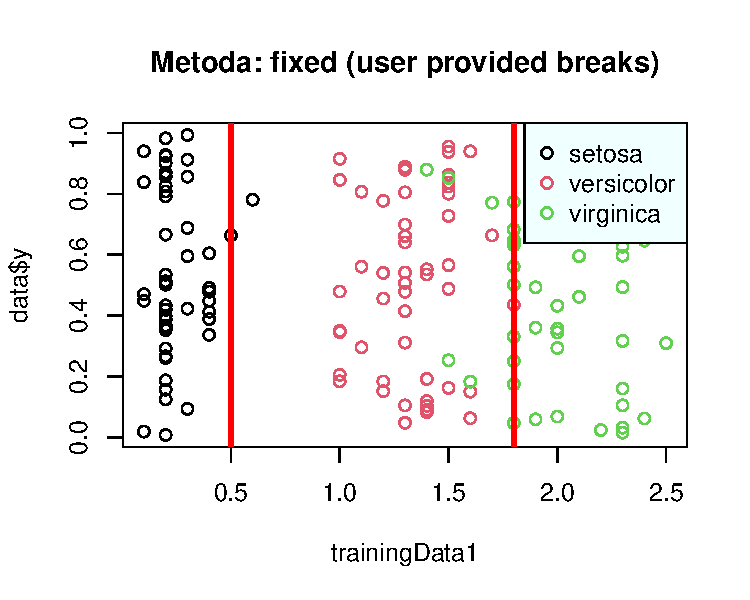
\includegraphics{Sprawozdanie2_files/figure-latex/givenRanges_najl-2} \end{center}

\begin{center}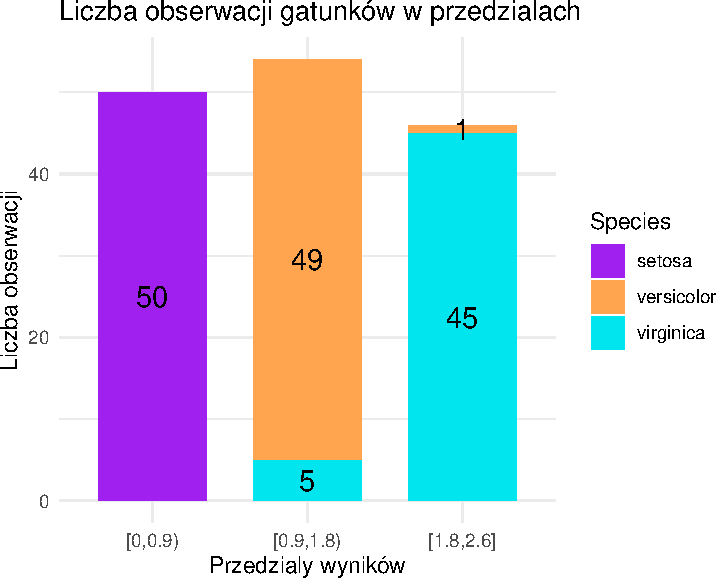
\includegraphics{Sprawozdanie2_files/figure-latex/tabela_kondygnacji_4_najl-1} \end{center}

\begin{verbatim}
##      [,1]
## [1,] 0.96
\end{verbatim}

\paragraph{Dla najgorszej}\label{dla-najgorszej-3}

\begin{center}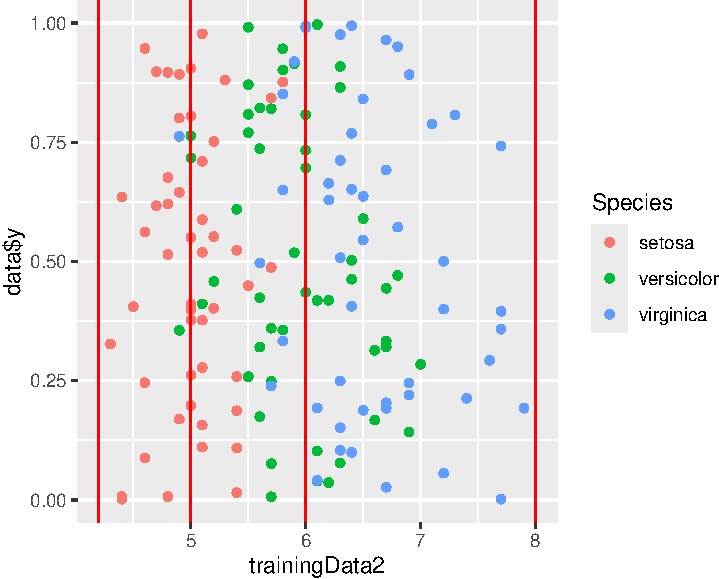
\includegraphics{Sprawozdanie2_files/figure-latex/givenRanges_najg-1} \end{center}

\begin{center}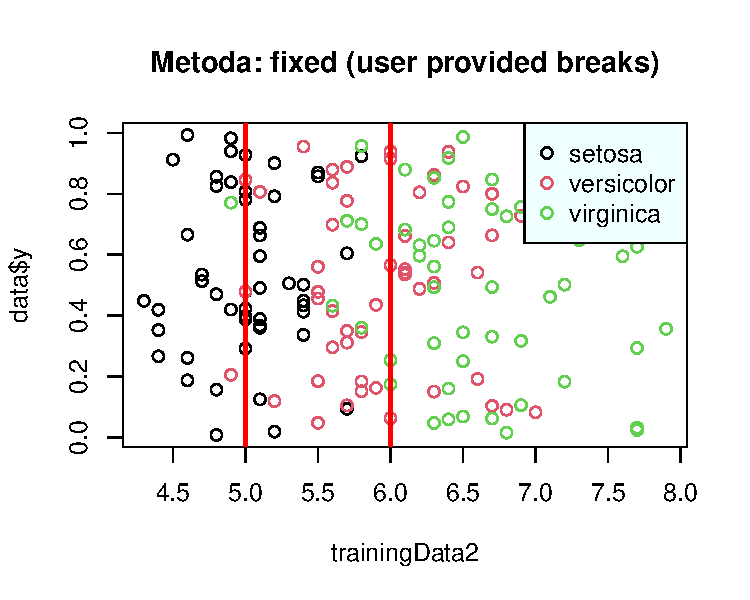
\includegraphics{Sprawozdanie2_files/figure-latex/givenRanges_najg-2} \end{center}

\begin{center}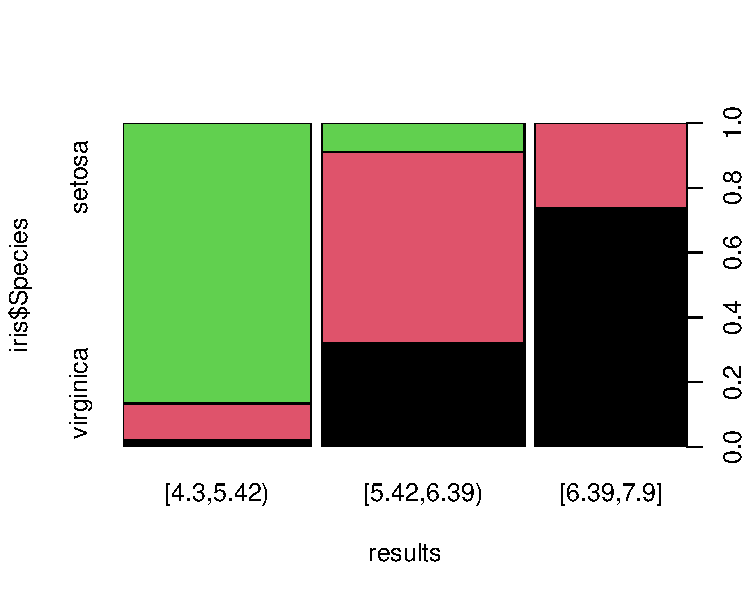
\includegraphics{Sprawozdanie2_files/figure-latex/tabela_kondygnacji_4_najg-1} \end{center}

\begin{verbatim}
##      [,1]
## [1,] 0.72
\end{verbatim}

\section{ZADANIE 2 (Analizaskładowych głównych (Principal Component
Analysis
(PCA)))}\label{zadanie-2-analizaskux142adowych-gux142uxf3wnych-principal-component-analysis-pca}

\subsection{a) Dane: City Quality of Life Dataset (plik
uaScoresDataFrame.csv, źródło:
Kaggle/Teleport.org)}\label{a-dane-city-quality-of-life-dataset-plik-uascoresdataframe.csv-ux17aruxf3dux142o-kaggleteleport.org}

\subsection{b) Przygotowanie danych}\label{b-przygotowanie-danych}

\subsection{c) Wyznaczenie składowych
głównych}\label{c-wyznaczenie-skux142adowych-gux142uxf3wnych}

\subsection{d) Zmienność odpowiadająca poszczególnym
składowym}\label{d-zmiennoux15bux107-odpowiadajux105ca-poszczeguxf3lnym-skux142adowym}

\subsection{e) Wizualizacja danych
wielowymiarowych}\label{e-wizualizacja-danych-wielowymiarowych}

\subsection{f) Korelacja zmiennych}\label{f-korelacja-zmiennych}

\subsection{g) Końcowe wnioski}\label{g-koux144cowe-wnioski}

\section{ZADANIE 3 (Skalowaniewielowymiarowe (Multidimensional Scaling
(MDS)))}\label{zadanie-3-skalowaniewielowymiarowe-multidimensional-scaling-mds}

\subsection{a) Dane: titanic\_train (R-pakiet
titanic)}\label{a-dane-titanic_train-r-pakiet-titanic}

\subsection{b) Przygotowanie danych}\label{b-przygotowanie-danych-1}

\subsection{c) Redukcja wymiaru na bazie
MDS}\label{c-redukcja-wymiaru-na-bazie-mds}

\subsection{d) Wizualizacja danych}\label{d-wizualizacja-danych}

\end{document}
